\section{Greedy Dynamic Quadruped Gait Generation}

\subsection{Terrain Representation}

\begin{outline}
  Explain how you represent the terrain for CNN input.
\end{outline}

%%%%%%%%%%%%%%%%%%%%%%%%%%%%%%%%%%%%%%%%%%%%%%%%%%%%%%%%%%%%%%%%%%%%%%%%%%%%%%%%%%%%%%%%%%%%%%%%%%%%
\subsection{Network Architecture}

\begin{outline}
  Detail the architecture of the CNNs used for contact configuration
  and footstep target/swing duration evaluation.
\end{outline}

The footstep evaluation neural network architecture is shown in
\autoref{fig:diagram-contactnet-architecture} accomplishes a similar
task to ContactNet \cite{bratta_contactnet_2024}. It takes in terrain
and state information and ranks each of the possible footstep
positions. This network uses a multi-modal middle fusion
architecture. This architecture was chosen to effectively combine the
spatial features from the terrain data with the contextual features
from the robot state data, while still maintaining flexibility in
case re-training is needed \cite{feng2021deep}. The terrain data is
processed through a convolutional layer and fully connected layer,
while the robot state data is processed through fully connected
layers. The outputs of these two branches are then concatenated and
passed through an additional fully connected layer to produce the
final output, which consists of preference ratings for each potential
footstep position.

\begin{figure}
  \centering
  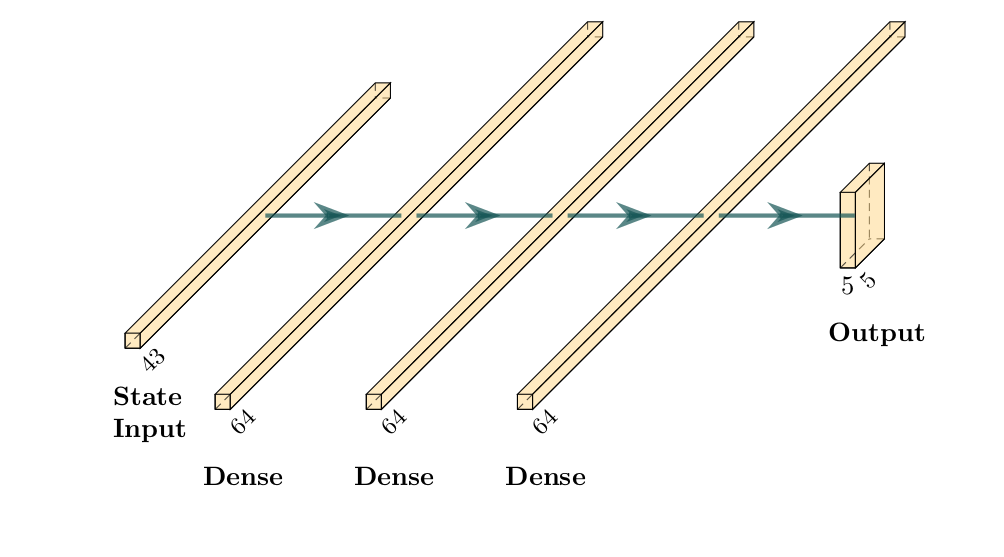
\includegraphics[width=0.5\linewidth]{images/diagrams/contact-network-architecture.png}
  \caption{Footstep evaluation neural network architecture.}
  \label{fig:diagram-contactnet-architecture}
\end{figure}

The footstep evaluation network is then used to feed the gait net
architecture shown in \autoref{fig:diagram-gaitnet-architecture}. The
gait net takes in the robot state information and ranked footstep
positions from the footstep evaluation network. It then outputs the
desired contact state\textemdash which feet should be in contact with
the ground. This information is then passed as constraints to the MPC.

\begin{figure}
  \centering
  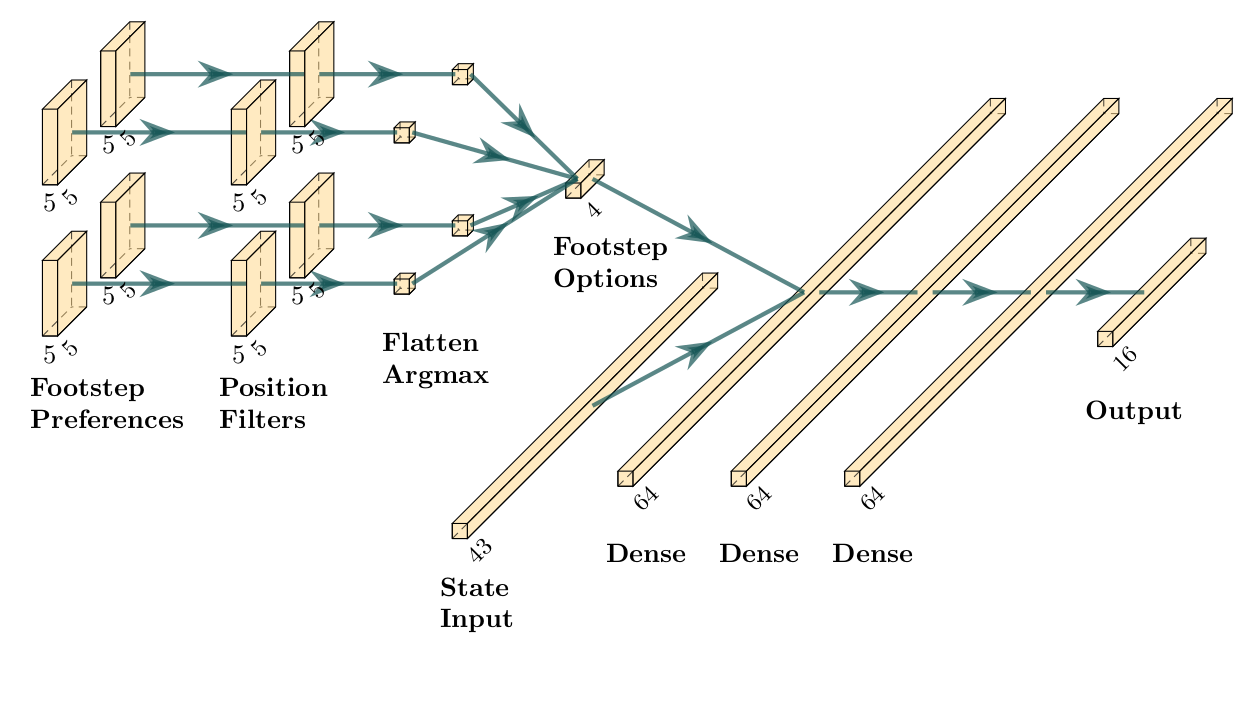
\includegraphics[width=0.5\linewidth]{images/diagrams/gait-network-architecture.png}
  \caption{Gait net architecture.}
  \label{fig:diagram-gaitnet-architecture}
\end{figure}

\begin{todo}
  Discuss gait net architecture
\end{todo}

\begin{todo}
  Discuss training procedure
\end{todo}

%%%%%%%%%%%%%%%%%%%%%%%%%%%%%%%%%%%%%%%%%%%%%%%%%%%%%%%%%%%%%%%%%%%%%%%%%%%%%%%%%%%%%%%%%%%%%%%%%%%%
\subsection{Greedy Decision-Making}

\begin{outline}
  Elaborate on the greedy selection process for choosing the
  highest-scoring, feasible action.
\end{outline}
